\section{Ownership Assignment}
\label{section:ownership}

We formulate the last-mile search problem in terms of \textit{locations}, which are searchable entities that 'own' or contain any number of \textit{objects}. %(i.e., a location that contains <object1, object2, etc.>, or a location that contains <object1 Northeast of object2>). 
To support user queries, \emph{GESTALT} must associate objects with their parent locations.
We call this problem \textit{Object Ownership Assignment} and define it as follows.
Given a collection of locations and objects within a region, \emph{Ownership Assignment} seeks to assign each object to its 'parent' location correctly. 
Ownership Assignment amounts to a clustering problem where points (objects) are assigned to centroids (locations) that are known apriori. 
The objects are not uniformly distributed across locations, and some locations may not have associated tagged objects. 

Further, the human eye does not see the world in regular grid lines like on a map. Hence, the ownership assignment process is naturally inexact, and objects are 'shared' between locations where appropriate.
For example, a winery may have a shed out back that is visible both from that winery and a neighboring one. 
In this case, the object can be helpful when searching for either location. 
We address this aspect of the problem by modifying our method to allow for fuzzy object-location assignment, effectively increasing the recall of the method. 

\subsection{Datasets and Metrics}

We evaluate the Ownership Assignment task on two datasets: the hand-labeled Swan Valley Wineries dataset alone and a \textit{Combined} dataset that includes all of the object and location tags from the Swan Valley Wineries dataset and the noisy object tags from the Flickr dataset and crowd-sourced object tags from the OSM dataset.
Since we have ground truth labels for the winery locations and their objects in the Wineries dataset, we report both precision and recall on this dataset.
The Combined dataset presents a more realistic and challenging scenario for Ownership Assignment than the Wineries dataset alone, given its more extensive set of locations and large set of object tags to assign. However, since the Combined dataset includes noisy tags for which we have no ground truth labels, we do not report precision on the Combined dataset. Instead, we measure the recall of object assignment to the labeled Winery locations. The Combined dataset tests how well the recall performance of our Ownership Assignment method holds up to additional noise and more densely packed objects and locations.
The Swan Valley Wineries dataset consists of 31 wineries and 5 breweries and 146 objects hand-labeled across 6 of those locations with ground-truth labels. Table \ref{table:clustering} contains the recall (and precision, where applicable) on those locations and objects.

\subsection{Method}

Our method for Object Ownership Assignment is outlined in Algorithm \ref{alg:OwnershipAssignment}. 
After clustering the objects, we determine the centroids of the relevant object clusters, calculate the confidence scores in the object-cluster assignments, and then map the cluster centroids to their nearest known location tags. 
When calculating the confidence scores, we normalize the object-centroid distances (omitting objects in the null cluster, which has no meaningful centroid and would skew the normalization). 
This confidence score (between 0 and 1) measures how far a given object is from its cluster's centroid, assigning higher scores to objects near the centroid and lower ones to objects far from the centroid. 
We take this approach rather than using a static threshold parameter (like within x distance) to account for the variety in object density of the region under search. 
We adopt the convention of assigning null cluster objects a confidence score of 0.5 since these objects are deemed to be noise and are not relevant or helpful in finding locations.
To further account for uncertainty in object tags, we add an adjustable parameter \textit{c} to the method, which allows for a varying degree of \textit{fuzzy assignment} of objects to clusters. 
By increasing the parameter value, we can allow for objects to be assigned to multiple clusters if they are close to the centroid (within \textit{$c\%$} of the largest object-centroid distance in the dataset, the same value used to normalize the confidence scores). %We 

\begin{algorithm}
    \caption{Object to Location Ownership Assignment Algorithm}
    \label{alg:OwnershipAssignment}
    \begin{algorithmic}
        \State{\textit{\textbf{Locs}} a list of locations and their tagged coordinates}
        \State{\textit{\textbf{Objs}} a list of objects and their coordinates}
        \State{\textit{\textbf{Clusters}} a list of object clusters}
        %\State{\textit{\textbf{C}} an individual cluster in $Clusters$}
        %\State{\textit{\textbf{C.x}} a cluster centroid}
        \State{\textit{\textbf{C.l}} the predicted $location$ for a $cluster$}
        %\State{\textit{\textbf{O}} an individual object in $Objects$}
        \State{\textit{\textbf{O.c}} confidence score that object was correctly assigned}
        %\State{\textit{\textbf{O.x}} an object's coordinates}
        \State{- - - - - - - - - -}
        \Procedure{ObjectOwnershipAssignment}{$Locs$,$Objs$}
            \State{$Clusters\leftarrow$ \textbf{DBSCAN}($Objs$)}%\Comment{\textbf{C}luster}
            \For{All $C$ in $Clusters$ except NULL cluster}
                \State{$C.x\leftarrow$ Calculate Cluster Centroid}%\Comment{$C.x$ cluster centroid}
                \For{$O$ in $C$}
                    \State{$O.c\leftarrow$ $1-normalize(dist(O,C.x)$}%\frac{1}{dist(O, C.x)}$}%\Comment{\textbf{O}bj \textbf{C}onf, $O.x$ obj coords}
                \EndFor
            \EndFor
            \For{All $O$ in NULL Cluster}
                \State{$O.c\leftarrow$ 0.5}
            \EndFor
            \For{All $C$ in $Clusters$ Except NULL Cluster}
                \State{$C.l\leftarrow$ Closest $L$ in $Locs$ to $C.x$}%\Comment{\textbf{C}luster \textbf{L}oc, $L.x$ Loc coords}
            \EndFor 
        \EndProcedure
    \end{algorithmic}
\end{algorithm}

%\subsection{Results} \label{subsection:own_results}
We run all Swan Valley Wineries experiments with DBSCAN parameter $\epsilon = \frac{0.05}{6371}$ and later Washington D.C. experiments with $\epsilon = \frac{0.01}{6371}$. For both regions we set the MinClusterSize=$3$. These parameters were selected using the knowledge about the general setting for each dataset, with Swan Valley being a semi-rural environment and Washington D.C. being a dense urban environment. For Swan Valley, the epsilon value is set to the equivalent of roughly 50m	, a reasonable cluster neighborhood size for such an environment. Generally, the minClusterSize is not critical given that fuzzy assignment allows objects to be added to nearby clusters, which overcomes too fine a clustering outcome. 


\small{
\begin{table}[h!]
    \begin{center}
        \begin{tabular}{ |c|c|c|c|c| } 
            \hline
            Dataset & Method & Fuzzy Param & Precision & Recall \\
            \hline
            \multirow{5}{4em}{Swan Valley Wineries} 
                & Exact & $c = 0$ & $1.0$ & $0.89$  \\ 
                & Fuzzy & $c = 2$ & $0.85$ & $0.89$  \\ 
                & Fuzzy & $c = 4$ & $0.85$ & $0.89$  \\
                & Fuzzy & $c = 6$ & $0.85$ & $0.89$  \\ 
                & Fuzzy & $c = 8$ & $0.85$ & $0.89$  \\ 
                & Fuzzy & $c = 10$ & $0.85$ & $0.89$  \\ 
            \hline
            \multirow{5}{4em}{Combined} 
                & Exact & $c = 0$ & - & $0.88$  \\ 
                & Fuzzy & $c = 2$ & - & $0.88$  \\ 
                & Fuzzy & $c = 4$ & - & $0.91$  \\ 
                & Fuzzy & $c = 6$ & - & $0.94$  \\ 
                & Fuzzy & $c = 8$ & - & $0.97$  \\ 
                & Fuzzy & $c = 10$ & - & $0.98$  \\ 
            \hline
        \end{tabular}
        \caption{ Object-to-location assignment results for Swan Valley Wineries and Combined datasets. Increasing fuzziness improves recall on the noisier \textit{Combined} dataset.} %increases the chance objects are assigned to multiple clusters, which
        \label{table:clustering}
    \end{center}
\end{table}
}


\subsection{Results}
We show the Object-to-location assignment results for the Swan Valley Wineries and the \textit{Combined} datasets in Figure \ref{table:clustering}. 
Increasing the fuzziness parameter $c$ increases the chance that objects are assigned to multiple clusters, which improves recall on the noisier \textit{Combined} dataset.
As expected, increasing the likelihood that objects are assigned to multiple clusters in the less noisy Swan Valley Wineries dataset reduces the precision but, does not show the benefit in recall that it did for the noisier \textit{Combined} dataset.

Overall, the object ownership results show that our method, while straightforward, handles the noisy object tags well, especially on the larger dataset. By using DBSCAN for the initial clustering, we observe a noise reduction effect as objects which do not belong to any locations are relegated to the NULL cluster (i.e., a mistagged singular object with nothing else around it for miles in any direction), and a similar recall on the ground-truth labels is achieved despite adding a considerable quantity of noisy object tags (in the \textit{Combined} dataset). 

The downside of using DBSCAN in this context is that it determines the centroids of the object clusters based on the object density, and then we must map those to our known location centroids in a post-processing step. 
Ideally, a better solution would start with the centroids and cluster around them while retaining the noise reduction effects of DBSCAN.
We leave a detailed comparison of Object Ownership Assignment techniques as an interesting avenue of future study for the last-mile search problem.



%In the absence of reliable crowd-sourced data linking objects to their parent locations, the ownership assignment problem necessitates an unsupervised solution to scale to any nontrivial number of locations and objects. 

%\osullikomment{Might it be worth bringing the shawshank quote right up to the front? It's really good - shows locations, finding things on geospatial relations, and has a fun pop culture hook element too}
%Recall the famous line from \textit{The Shawshank Redemption}\footnote{\href{https://www.imdb.com/title/tt0111161/}{https://www.imdb.com/title/tt0111161/}} \textit{"There’s a big hayfield up near Buxton... It’s got a long rock wall with a big oak tree at the north end ... At the base of that wall, 	u’ll find a rock that has no earthly business in a Maine hayfield. Piece of black, volcanic glass.”}. 
%Real people, in the real world don't think, or remember by latitude and longitude. 
%They live in the world, and experience it thorugh the things that they can see, hear, touch, smell and taste. 
%We design \emph{GESTALT} to enable users to search for locations using the same intuitive tools and tecniques that one might use to tell a friend how to get to a camping site they like, or, in Andy Dufrense's case, where Red can find buried treasure. 
%We enable users to use their experiences of locations in the real world as the search conditions (i.e. a location that contains <object1, object2, etc.>, or a location that contains <object1 Northeast of object2>). 

%discuss how changing this parameter affects the precision and recall in subsection \ref{subsection:own_results}.
%In step 6: Given a KD tree constructed from location point coordinates, a nearest neighbor search on the KD tree yields the location nearest to the centroid and it is assigned ownership of that cluster
%\subsection{Method- Fuzzy Object Ownership Assignment} 
%..................TODO NSCH:............ Write up ALGO for fuzzy clustering of objects to locations, where objects can be assigned to multiple locations with some probability p.
%Of note, because the human eye can see over property boundaries and other invisible lines on maps, we can accept a small margin of error where objects from neighboring locations might be mislabeled. For example, perhaps there is a large red shed at the back of a location's property that is not visible to the main part of the parent location but is clearly visible to the neighboring location.
%There will also exist some objects which plausibly could be seen and remembered by patrons of several locations, for example, a lake or a giant statue. 

%\begin{figure*}[ht]
%\label{fig:cmeans}        
%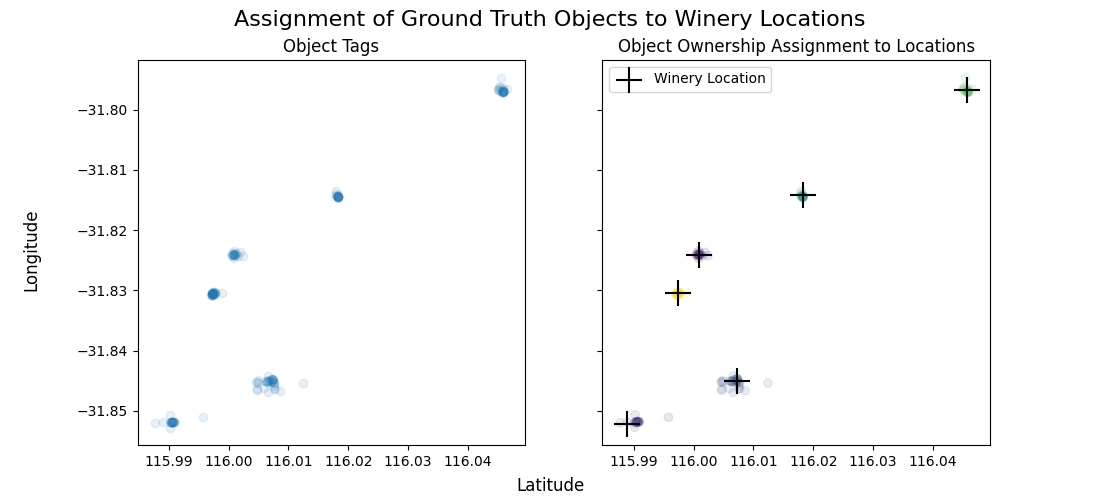
\includegraphics[width=\textwidth]{gestalt_cmeans.png}
%\centering
%\caption[width=\textwidth]{............}
%\end{figure*}



%\osullikomment{DVBSCAN doesn't do what I thought it did. I think one for future work is modifying DBSCAN to start with known possible centroids (or cluster seeds)}
%The DVBSCAN algorithm Ram et al. proposed in 2010 presents a promising direction to resolve this problem~\cite{Ram2010}, while retaining the noise reduction effects of traditional DBSCAN. 


%\subsection{Scalability}
%The ownership assignment process needs to be unsupervised to enable scaling to millions of object tags. 





%Examining the errors reveals the following insights about each clustering technique. 
%\textbf{When K-Means clusters incorrectly, labels are still correct.} When $K$ exceeds the number of clusters, it fragments the actual clusters. 
%However, in ideal conditions like the Wineries Dataset, where locations are separated, the centroids of these cluster fragments are still closest to the correct location. 
%As a consequence, they are correctly labeled despite being incorrectly clustered. We expect the accuracy will drop when locations are more densely packed. However, when we aim to process all objects and locations in a region concurrently, the number of clusters will likely approach the number of locations, and the issue will be less pronounced. 


%The second, more common (and more challenging approach) formulates an unsupervised learning problem using clustering libraries from \textit{scikit-learn}\footnote{\href{https://pypi.org/project/scikit-learn/}{Scikit-Learn PyPI Repo}}. 

%Ownership assignment is the unsupervised process through which objects are associated with locations. 
%Objects need to be associated with locations in \textit{GESTALT} because for the \textit{concept mapping} process and \textit{search} subsystem to work, they need to know which objects belong to each location.
%For example, assuming two adjacent wineries, a fountain between them would be west of one but east of the other. The mapping will be incorrect unless it is clear which winery it belongs to. 
%Similarly, for search, the underlying idea for \textit{GESTALT} is that people will remember particular objects at locations and use them as clues to find them again. Without an accurate object-to-location assignment, the search functionality will not work. 
 
%The Ownership Assignment process accepts two inputs, a collection of locations with their coordinates and a collection of objects with their coordinates. 
%The process works to assign each object to its parent location. 
%The process ends when objects are mapped to their parent locations. 